
\subsection{Sparse Distributed Representation}
% \subsection{The Datastructure of the Brain}


\begin{frame}[c,fragile]{Data Saving - Computer Science Solution}
    \Large
    What is \verb|01100101|? \pause Could be either one of:
    % What is ? Could be:
    \begin{itemize}[<+(1)->]
        \item Booleans (\verb|False, True, True, False,|\dots)
        \item Integer (\verb|101|)
        \item Float (\verb|3328.0|)
        \item (Byte-) String (\verb|'e'|)
        \item Pointer to something else
        \item Part of some other Datastructure
    \end{itemize}
\end{frame}


\begin{frame}[c,standout]
    Biological observation: \newline
    We use only part of our brain!
\end{frame}


\begin{frame}[c]{Sparse Distributed Representation - Introduction}
    \Large
    \begin{itemize}[<+(1)->]
        \item Datastructure of the brain
        \item Sparse (around 2\% are active)
        \item Distributed (clusters are somewhat rare)
        \item Inhibitory mechanisms
        \item Neuron states actually have 'meaning'
        \item Combined, they give context as well
        \item Many mechanisms in the brain would not work otherwise
    \end{itemize}
\end{frame}


\begin{frame}[c]{Sparse Distributed Representation - Example}
    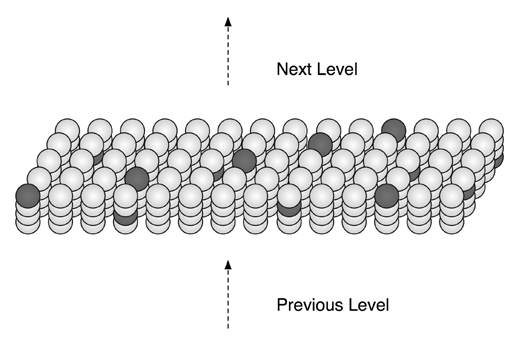
\includegraphics[width=0.95\textwidth]{region_sparse}
\end{frame}


\begin{frame}[c]{Sparse Distributed Representation - Example}
    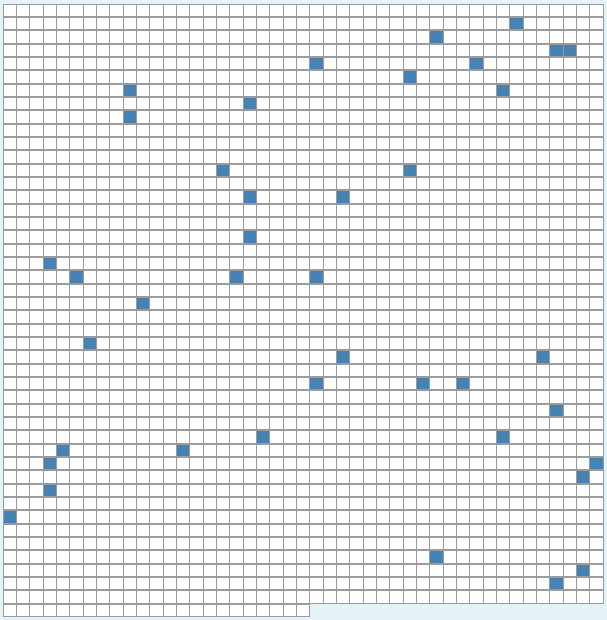
\includegraphics[height=0.9\textheight]{sdr_example}
\end{frame}

% \begin{frame}[c]
    % 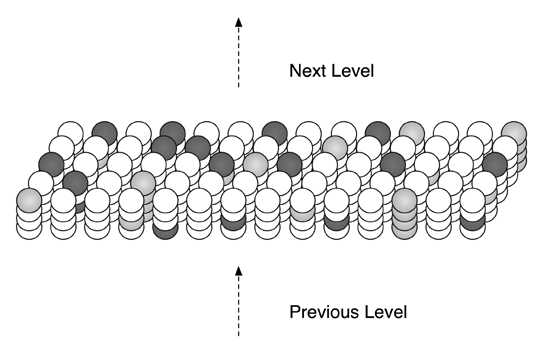
\includegraphics[width=0.9\textwidth]{region_predict}
% \end{frame}


\begin{frame}[c,standout]
    Live Demo!
\end{frame}


\begin{frame}[c]{Sparse Distributed Representation - Live Demos}
    \Large
    \begin{itemize}[<+(1)->]
        \item Ep2/Capacity
        \item Ep2/Matching (Noise resistency)
        \item Ep3/Subsampling
        \item Ep4/Classification
        \item Ep4/Union
        \item Ep5/Scalar Encoding
        \item Ep6/Date Encoding
        \item Ep5/RDSE - Number Encoding
    \end{itemize}
\end{frame}


\begin{frame}[c]{Encoders - Conclusion}
    \begin{itemize}[<+(1)->]
        \item Semantically similar data should result in SDRs with overlapping active bits.
        \item The same input should always produce the same SDR as output.
        \item The output should have the same dimensionality (total number of bits) for all inputs.
        \item The output should have similar sparsity for all inputs and have enough one-bits to handle noise and subsampling.
    \end{itemize}

    \normalsize
    \pause
    Cited from \cite{hawkins2016book}.
\end{frame}

